

\subsection{mavros发送offboard数据流}
\begin{lstlisting}[title=publish messgae, frame=shadowbox]
    // 1. offboard publish (mavros topic)
    fixed_wing_local_att_sp_pub = nh.advertise<mavros_msgs::AttitudeTarget>("mavros/setpoint_raw/attitude", 10);
    
    #define MAVLINK_MSG_ID_SET_ATTITUDE_TARGET 82
      typedef struct __mavlink_set_attitude_target_t {
          uint32_t time_boot_ms; /*< [ms] Timestamp (time since system boot).*/
          float q[4]; /*<  Attitude quaternion (w, x, y, z order, zero-rotation is 1, 0, 0, 0)*/
          float body_roll_rate; /*< [rad/s] Body roll rate*/
          float body_pitch_rate; /*< [rad/s] Body pitch rate*/
          float body_yaw_rate; /*< [rad/s] Body yaw rate*/
          float thrust; /*<  Collective thrust, normalized to 0 .. 1 (-1 .. 1 for vehicles capable of reverse trust)*/
          uint8_t target_system; /*<  System ID*/
          uint8_t target_component; /*<  Component ID*/
          uint8_t type_mask; /*<  Mappings: If any of these bits are set, the corresponding input should be ignored: bit 1: body roll rate, bit 2: body pitch rate, bit 3: body yaw rate. bit 4-bit 6: reserved, bit 7: throttle, bit 8: attitude*/
     }) mavlink_set_attitude_target_t;
\end{lstlisting}
\section{Coordinated Turn 协调转弯}
\subsection{not being wind}
方向角的变化率是和机体的roll以及倾斜角(bank angle)有关系, 我们需要寻找一个简单的关系来帮助我们研究这种线性传递函数的关系 -- 协调转弯. \par
在协调转弯期间, 飞机在体坐标系下没有横向加速度. 从分析的角度来看, 协调转弯的一个假设运行我们得到一个简单的表达式将 heading rate 和 bank angle 联系起来. \par
协调转弯时, 为了无人机没有侧向力, bank angle $\phi$ 被设置.
在图\ref{fig:1}中, 作用在微型飞行器上的离心力与作用在水平方向上的升力的水平分量相等并相反。
\begin{figure}[htpb]
    \centering
    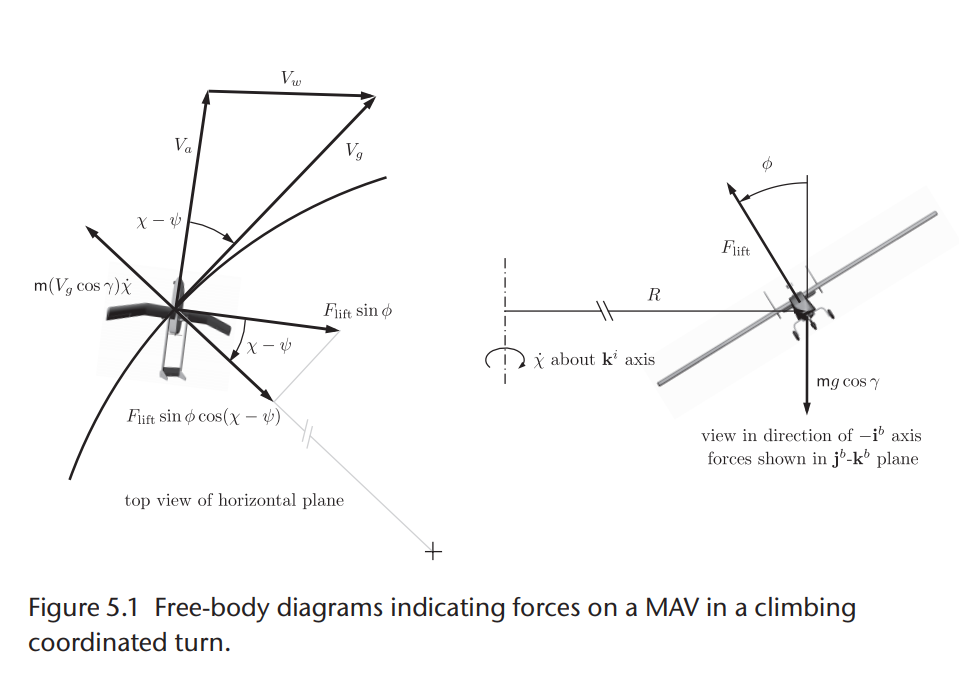
\includegraphics[width=0.8\textwidth]{pictures/5_1.png}
    \caption{爬升协调转弯MAV上的力}
    \label{fig:1}
\end{figure}
\par 作用在水平方向力的关系表示如下: 
\begin{align}
    F_{lift} sin \phi cos (\chi - \psi) &= m \frac{v^{2}}{R} \nonumber \\
    &= m v \omega \nonumber \\
    &= m (V_{g} cos \gamma) \dot{\chi} 
    \label{equ:1}
\end{align}
其中, $F_{lift}$代表的是升力, $\gamma$ 代表的是飞行轨迹的角度, $V_{g}, \chi$ 分别表示的是地速度以及方向角. \textcolor{red}{向心加速度的表达式: $a_{n} = \frac{v^{2}}{R} = v \omega$}
\par 离心力(The centrifugal force)(\textcolor{red}{$m (V_{g} cos \gamma) \dot{\chi} $})计算的时候, 用到了在惯性坐标系$k^{i}$上的方向角变化率$\dot{\chi}$ 和 速度的水平分量 $V_{a}cos \gamma$
\par 同样, 升力的垂直分量与重力在 $j^{b} - k^{b}$平面上的投影是等大反向的. 
垂直方向上的合力为:
\begin{equation}
    F_{lift} cos \phi = mg cos\gamma
    \label{equ:2}
\end{equation}
将等式\ref{equ:1}除以\ref{equ:2}得的 $\dot{\chi}$
\begin{equation}
    \dot{\chi} = \frac{g}{V_{g}} tan \phi cos(\chi - \psi)
    \label{equ:3}
\end{equation}
等式\ref{equ:3}就是协调转弯的表达式. 
\par 考虑到转弯半径等于 \textcolor{blue}{ $R = V_{g} \frac{cos \gamma}{\dot{\chi}}$}, 将上式代入半径中, 得到式子\ref{equ:4}. 在没有风或侧滑的情况下, 有\textcolor{red}{$V_{a} = V_{g}$和$\psi = \chi$}, 从而得到了式子\ref{equ:5}. 
\begin{equation}
    R = \frac{V_{g}^{2} cos \gamma}{g tan \phi cos(\chi - \psi)} 
    \label{equ:4}
\end{equation}
\begin{equation}
    \dot{\chi} = \frac{g}{V_{g}} tan \phi = \dot{\psi} = \frac{g}{V_{a}} tan \phi
    \label{equ:5}
\end{equation}
\par 在 9.2 节中, 我们将要介绍 在有风的情况下 \textcolor{blue}{$ \dot{\psi} = \frac{g}{V_{a}} tan \phi$} 该式子也成立
\clearpage
\subsection{being wind-Kinematic Model of Controlled Flight}
% 控制飞行动力学模型\par
在推导降阶表达式中, 简化的目的是估计运动中力平衡以及动量平衡的关系式(这些包含了 $\dot{u}, \dot{v}, \dot{\omega}, \dot{p}, , \dot{q}, \dot{r}$), 预估这些变量需要计算复杂的空气动力. 这些变量表达式可以被更简单的动力学表达式替代. 
这个更简单的动力学表达式是\textcolor{blue}{针对协调转弯和加速爬升的特定飞行条件而导出}.
\begin{figure}[htpb]
    \centering
    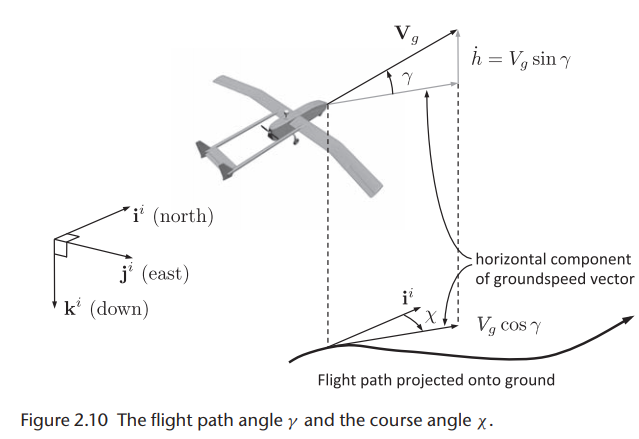
\includegraphics[width=0.8\textwidth]{pictures/2_10.png}
    \caption{航线轨迹角度$\gamma$和航向角$\chi$}
    \label{fig:2_10}
\end{figure}
针对图\ref{fig:2_10}, 飞机相对于惯性系的速度矢量可以用航向角和(惯性参考)飞行路径角表示为 
\begin{gather} % 输入多行公式
    V_{g}^{i} = V_{g} \begin{pmatrix}
        cos \chi cos \gamma \\
        sin \chi cos \gamma \\
        -sin \gamma \\
      \end{pmatrix}
      = \begin{pmatrix}
        \dot{p_{n}} \\
        \dot{p_{e}} \\
        \dot{h} \\
      \end{pmatrix}
      \label{equ:6}
  \end{gather}
\par 由于控制飞机的航向和空速是很常见的,因此用$\psi$和$V_{a}$表示等式\ref{equ:6}很有用. 
\begin{gather} % 输入多行公式
    V_{g} \begin{pmatrix}
        cos \chi cos \gamma \\
        sin \chi cos \gamma \\
        -sin \gamma \\
      \end{pmatrix} - \begin{pmatrix}
        w_{n} \\
        w_{e} \\
        w_{d} \\
      \end{pmatrix} =  V_{a} \begin{pmatrix}
        cos \psi cos \gamma_{a} \\
        sin \psi cos \gamma_{a} \\
        -sin \gamma_{a} \\
      \end{pmatrix}
      \label{equ:wind}
  \end{gather}
  结合风的表达式\ref{equ:wind}(地速等于空速加风速, 
    其中的 $\gamma_{a}$ 代表的是 空速的方向和水平方向的夹角), 我们可以得到
  \begin{gather} % 输入多行公式
    \begin{pmatrix}
        \dot{p_{n}} \\
        \dot{p_{e}} \\
        \dot{h} \\
      \end{pmatrix} = V_{a} \begin{pmatrix}
        cos \psi cos \gamma_{a} \\
        sin \psi cos \gamma_{a} \\
        sin \gamma_{a} \\
      \end{pmatrix} +  \begin{pmatrix}
        w_{n} \\
        w_{e} \\
        -w_{d} \\
      \end{pmatrix}
      \label{equ:7}
  \end{gather}
  如果我们假设飞机保持在一个恒定的高度,并且没有向下的风分量,那么运动学表达式简化为\ref{equ:8}, 同样该模型也是无人机领域中比较常用的模型. 
  \begin{gather} % 输入多行公式
    \begin{pmatrix}
        \dot{p_{n}} \\
        \dot{p_{e}} \\
        \dot{h} \\
      \end{pmatrix} = V_{a} \begin{pmatrix}
        cos \psi \\
        sin \psi \\
        0 \\
      \end{pmatrix} +  \begin{pmatrix}
        w_{n} \\
        w_{e} \\
        0 \\
      \end{pmatrix}
      \label{equ:8}
  \end{gather}
  \subsection{Coordinated Turn}
  之前的协调转弯的表达式为 $\dot{\chi} = \frac{g}{V_{g}} tan \phi cos(\chi - \psi)$. 
  即使在第6章中描述的自动驾驶回路并没有强制执行协调转弯条件,
  飞机必须倾斜才能转弯(而不是打滑才能转弯)这个基本条件已经被这个模型捕捉到了。\par
  协调转弯可以被 heading 和 空速进行表示. 我们先对\ref{equ:wind}两边进行求导, 得到下面的式子\ref{equ:9}
  \begin{gather} % 输入多行公式
    \begin{pmatrix}
        cos \chi cos \gamma & - V_{g} sin \chi cos \gamma & - V_{g} cos \chi sin \gamma \\
        sin \chi cos \gamma & V_{g} cos \chi cos \gamma & - V_{g} sin \chi sin \gamma \\
        -sin \gamma & 0 & -cos \gamma \\
      \end{pmatrix} \begin{pmatrix}
        \dot{V_{g}} \\
        \dot{\chi} \\
        \dot{\gamma} \\
    \end{pmatrix}
      = \begin{pmatrix}
        cos \psi cos \gamma_{a} & - V_{a} sin \psi cos \gamma_{a} & - V_{a} cos \psi sin \gamma_{a} \\
        sin \psi cos \gamma_{a} & V_{a} cos \psi cos \gamma_{a} & - V_{a} sin \psi sin \gamma_{a} \\
        -sin \gamma_{a} & 0 & -cos \gamma_{a} \\
      \end{pmatrix} \begin{pmatrix}
        \dot{V_{a}} \\
        \dot{\psi} \\
        \dot{\gamma_{a}} \\
    \end{pmatrix}
      \label{equ:9}
  \end{gather}
  \par 在定高和没有向下风分量的情况下, $\gamma, \gamma_{a}, \dot{\gamma}, \dot{\gamma_a}$ 和 $w_{d}$ 都是0, 根据$\dot{V_{a}}$ 和$\dot{\chi}$求解$\dot{V_{g}}$ 和$\dot{\psi}$
  \begin{equation}
    \begin{split}
      \dot{V_{g}} &= \frac{\dot{V_{a}}}{cos (\chi - \psi)} + V_{g} \dot{\chi} tan(\chi - \psi) \\
      \dot{\psi} &= \frac{\dot{V_{a}}}{V_{a}} tan (\chi - \psi) + \frac{V_{g} \dot{\chi}}{V_{a}cos(\chi - \psi)}
    \end{split}
\end{equation}
\par 若假定空速为常数, 那么得\ref{equ:10} 最值得注意的是在有风的情况下,这个等式是成立的。
\begin{equation}
    \dot{\chi} = \frac{g}{V_{g}} tan \phi 
    \label{equ:10}
\end{equation}
\subsection{px4内部的实现}
第一次处理产生\ref{equ:att:turn:1}, 得到$roll_{constrained}$, 之后在对其进行$(-roll_{setpoint}, roll_{setpoint})$约束. 得出\ref{equ:att:turn:2}, 进而进行 PID 控制, 产生\ref{equ:att:turn:3}.
\begin{equation}
  roll_{constrained}=
  \begin{cases}
  constrained[-80^{o}, 80^{o}], &fabs(roll_{current} < 90^{o}) \\
  constrained[100^{o}, 180^{o}], &fabs(roll_{current} > 90^{o}) \& roll_{current} > 0^{o}\\
  constrained[-180^{o}, -100^{o}], &fabs(roll_{current} > 90^{o}) \&roll_{current} < 0^{o}
  \end{cases}
  \label{equ:att:turn:1}
\end{equation} \\
\begin{equation}
  roll_{constrained} =roll_{constrained}.constrained[-roll_{setpoint}, roll_{setpoint}]
  \label{equ:att:turn:2}
\end{equation}\\
\begin{equation}
  \begin{split}
    \dot{yaw} &= \frac{tan(roll_{constrained}) * cos(pitch_{current}) * G}{V_{air}} , (V_{air} = V_{air} < V_{air}^{min} ? V_{air}^{min} : V_{air}) \\
    \dot{roll} &= \frac{roll_{setpoint} - roll_{current}}{0.1} \\
    \dot{pitch} &= \frac{pitch_{setpoint} - pitch_{current}}{0.1}
    \label{equ:att:turn:3}
  \end{split}
\end{equation}
在第一次计算的基础上, 续进行第二手我们继计算, 在px4内部, 首先实现进行参数的设置(见下面的"参数设置"), 
\begin{equation}
  \begin{split}
  fw\_acro\_x\_max &= 90^{o} \\
  fw\_acro\_y\_max &= 90^{o} \\
  fw\_acro\_z\_max &= 45^{o}
  \end{split}
  \label{equ:config}
\end{equation}
\begin{lstlisting}[title=参数设置, frame=shadowbox]
  _roll_ctrl.set_max_rate(radians(_param_fw_acro_x_max.get()));
  _pitch_ctrl.set_max_rate_pos(radians(_param_fw_acro_y_max.get()));
  _pitch_ctrl.set_max_rate_neg(radians(_param_fw_acro_y_max.get()));
  _yaw_ctrl.set_max_rate(radians(_param_fw_acro_z_max.get()));
\end{lstlisting}
\begin{figure}[htbp]
  \centering
  \subfigure[x]{
      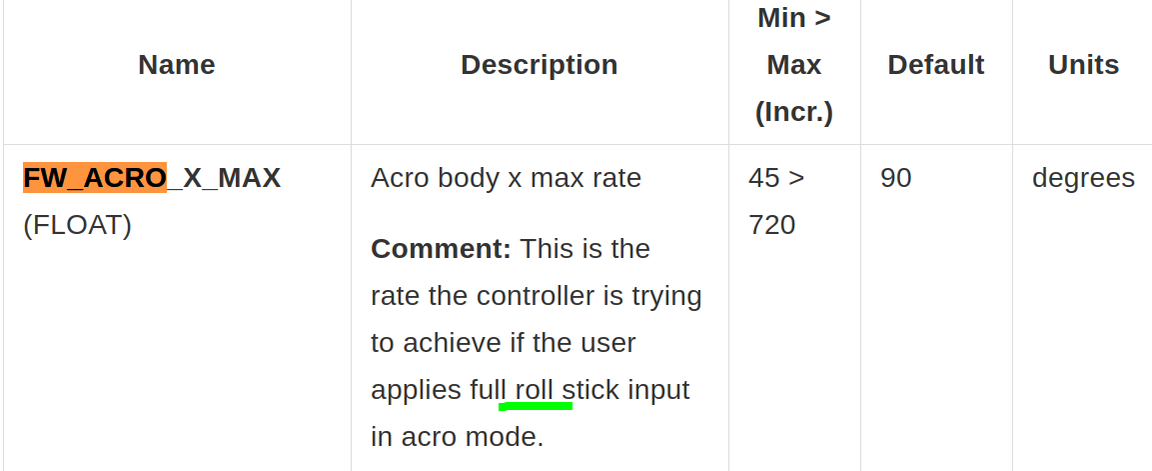
\includegraphics[width=0.48\textwidth]{pictures/parameter1.png}
  }
  \subfigure[y and z]{
      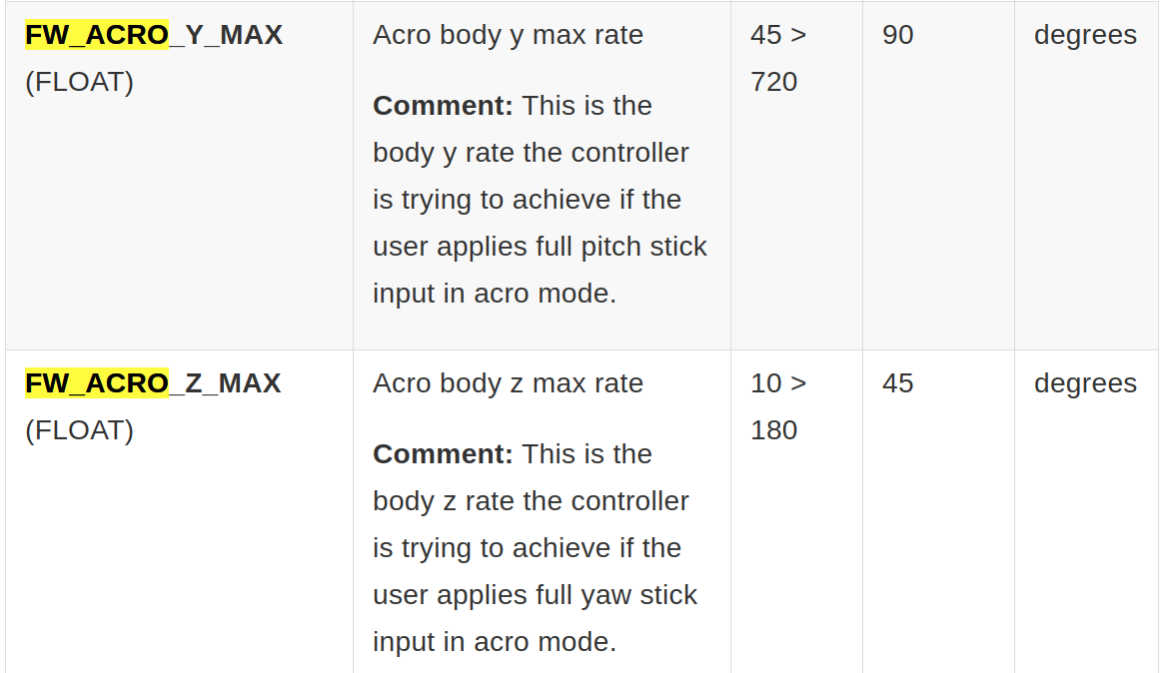
\includegraphics[width=0.48\textwidth]{pictures/att_parameter2.png}
  }
  \caption{parameters}
  \label{fig:param}
\end{figure}
其中各个参数的描述见\ref{fig:param}, 在px4中分别对应的值为\ref{equ:config}. 实现了各个参数的初始化之后, 进行下面的处理
\begin{equation}
  \begin{split}
  roll_{bodyrateSetpoint} &= [\dot{roll} - sin(pitch_{current}) * \dot{yaw}]\\
                          &.constrained[-FW\_ACRO\_X\_MAX, FW\_ACRO\_X\_MAX] \\    
  pitch_{bodyrateSetpoint} &= [cos(roll_{current})*\dot{roll} + cos(pitch_{current}) * sin(roll_{current}) * \dot{yaw}]\\
                          &.constrained[-FW\_ACRO\_Y\_MAX, FW\_ACRO\_Y\_MAX]\\
  yaw_{bodyrateSetpoint} &= [-sin(roll_{current}) * \dot{pitch} + cos(roll_{current}) * cos(pitch_{current}) * \dot{yaw}] \\
                          &.constrained[-FW\_ACRO\_Z\_MAX, FW\_ACRO\_Z\_MAX]
  \end{split}
\end{equation}
最终将上面约束过的体变化率当做姿态的设定值, 发布给下面的控制器以及执行器
\begin{equation}
  \begin{split}
    roll_{setpoint} &= roll_{bodyrateSetpoint} \\
    pitch_{setpoint} &= pitch_{bodyrateSetpoint} \\
    yaw_{setpoint} &= yaw_{bodyrateSetpoint}  
  \end{split}
\end{equation}
\subsection{欧拉角, 四元数的相互转换}
\subsubsection{欧拉角转换为四元数}

\begin{lstlisting}[title=欧拉角转换为四元数]
  void euler_2_quaternion(float angle[3], float quat[4])
  {
      // q0 q1 q2 q3
      // w x y z
      double cosPhi_2 = cos(double(angle[0]) / 2.0);
      double sinPhi_2 = sin(double(angle[0]) / 2.0);
      double cosTheta_2 = cos(double(angle[1]) / 2.0);
      double sinTheta_2 = sin(double(angle[1]) / 2.0);
      double cosPsi_2 = cos(double(angle[2]) / 2.0);
      double sinPsi_2 = sin(double(angle[2]) / 2.0);
      
      quat[0] = float(cosPhi_2 * cosTheta_2 * cosPsi_2 + sinPhi_2 * sinTheta_2 * sinPsi_2);
      quat[1] = float(sinPhi_2 * cosTheta_2 * cosPsi_2 - cosPhi_2 * sinTheta_2 * sinPsi_2);
      quat[2] = float(cosPhi_2 * sinTheta_2 * cosPsi_2 + sinPhi_2 * cosTheta_2 * sinPsi_2);
      quat[3] = float(cosPhi_2 * cosTheta_2 * sinPsi_2 - sinPhi_2 * sinTheta_2 * cosPsi_2);
  }  
\end{lstlisting}

\subsubsection{四元数转换为欧拉角}
\begin{lstlisting}[title=四元数转换为欧拉角]
  Quaternion(const Euler<Type> &euler)
    {
        Quaternion &q = *this;
    
        Type cosPhi_2 = Type(cos(euler.phi() / Type(2)));
        Type cosTheta_2 = Type(cos(euler.theta() / Type(2)));
        Type cosPsi_2 = Type(cos(euler.psi() / Type(2)));
        Type sinPhi_2 = Type(sin(euler.phi() / Type(2)));
        Type sinTheta_2 = Type(sin(euler.theta() / Type(2)));
        Type sinPsi_2 = Type(sin(euler.psi() / Type(2)));
        q(0) = cosPhi_2 * cosTheta_2 * cosPsi_2 +
               sinPhi_2 * sinTheta_2 * sinPsi_2;
        q(1) = sinPhi_2 * cosTheta_2 * cosPsi_2 -
               cosPhi_2 * sinTheta_2 * sinPsi_2;
        q(2) = cosPhi_2 * sinTheta_2 * cosPsi_2 +
               sinPhi_2 * cosTheta_2 * sinPsi_2;
        q(3) = cosPhi_2 * cosTheta_2 * sinPsi_2 -
               sinPhi_2 * sinTheta_2 * cosPsi_2;
}
\end{lstlisting}

\subsection{针对offboard对px4的更改}
在 \textcolor{red}{$fw\_att\_control.cpp$} 控制器中, 对yaw重新计算的时候, 使用的是 $roll_{setpoint}$ 而不是根据当前的roll进行两次约束之后得到的结果. 同时
也去掉$cos(pitch_{current})$这一项.
